% Author: Till Tantau
% Source: The PGF/TikZ manual
\documentclass[a4paper,11pt]{article}
\usepackage[utf8]{inputenc}
\usepackage{listings}
\usepackage{amsmath}    % need for subequations
\usepackage{graphicx}   % need for figures
\usepackage{verbatim}   % useful for program listings
\usepackage{color}      % use if color is used in text
%\usepackage{subfigure}  % use for side-by-side figures
\usepackage{hyperref}   % use for hypertext links, including those to external documents and URLs
\usepackage{url}
\usepackage{float}
\usepackage{todonotes}
\usepackage{tikz}
\usepackage{enumitem}
\usepackage{hyperref}
\usepackage{pdfpages}
\usepackage{caption}
\usepackage{subcaption}
\usepackage{listings}
\usepackage{color}
\usepackage{amsfonts}
\usepackage{latexsym}
\usepackage[T1]{fontenc} % use for allowing < and > in cleartext
\usepackage{fixltx2e}    % use for textsubscript
\usepackage[linesnumbered,boxed,ruled]{algorithm2e}
% \newcommand{\BigO}[1]{\ensuremath{\operatorname{O}\left(#1\right)}}
\newcommand{\BigO}[1]{\ensuremath{\mathop{}\mathopen{}\mathcal{O}\mathopen{}\left(#1\right)}}
\graphicspath{ {./images/} }
\definecolor{mygreen}{rgb}{0,0.6,0}
\definecolor{mygray}{rgb}{0.5,0.5,0.5}
\definecolor{mymauve}{rgb}{0.58,0,0.82}
\lstset{ %
  backgroundcolor=\color{white},   % choose the background color; you must add \usepackage{color} or \usepackage{xcolor}
  basicstyle=\footnotesize,        % the size of the fonts that are used for the code
  breakatwhitespace=false,         % sets if automatic breaks should only happen at whitespace
  breaklines=true,                 % sets automatic line breaking
  captionpos=b,                    % sets the caption-position to bottom
  commentstyle=\color{mygreen},    % comment style
  deletekeywords={...},            % if you want to delete keywords from the given language
  escapeinside={\%*}{*)},          % if you want to add LaTeX within your code
  extendedchars=true,              % lets you use non-ASCII characters; for 8-bits encodings only, does not work with UTF-8
  %frame=single,                    % adds a frame around the code
  keepspaces=true,                 % keeps spaces in text, useful for keeping indentation of code (possibly needs columns=flexible)
  keywordstyle=\color{blue},       % keyword style
  language=Octave,                 % the language of the code
  morekeywords={*,...},            % if you want to add more keywords to the set
  numbers=left,                    % where to put the line-numbers; possible values are (none, left, right)
  numbersep=5pt,                   % how far the line-numbers are from the code
  numberstyle=\tiny\color{mygray}, % the style that is used for the line-numbers
  rulecolor=\color{black},         % if not set, the frame-color may be changed on line-breaks within not-black text (e.g. comments (green here))
  showspaces=false,                % show spaces everywhere adding particular underscores; it overrides 'showstringspaces'
  showstringspaces=false,          % underline spaces within strings only
  showtabs=false,                  % show tabs within strings adding particular underscores
  stepnumber=2,                    % the step between two line-numbers. If it's 1, each line will be numbered
  stringstyle=\color{mymauve},     % string literal style
  tabsize=2,                       % sets default tabsize to 2 spaces
  %title=\lstname                   % show the filename of files included with \lstinputlisting; also try caption instead of title
}

\bibliographystyle{plain}
\begin{document}

\date{April 23rd 2014\\ IT University of Copenhagen}
\title{Homographies, Textures, Projections and Augmentations\\SIGB Spring 2014}

\author{Marcus Gregersen\\
\texttt{mabg@itu.dk}
\and Martin Faartoft\\
\texttt{mlfa@itu.dk}
\and Mads Westi\\
\texttt{mwek@itu.dk}}
\clearpage\maketitle
\thispagestyle{empty}
\setcounter{page}{1}
\newpage

\section{Introduction}
In this report we will experiment with homographies, texture mapping, projections and image augmentation. The report is divided into two parts. In the first part we cover homographies (\ref{sec:person}) and texture mapping (\ref{sec:linear}). In the second part we focus on projections and augmentation (\ref{sec:aug}).

\section{Person Location on Map}
\label{sec:person}
In this section, we will take a video of a person walking around the ITU atrium, and map his movement onto an overview map of the ITU building. This effectively eliminates the perspective, and allows for easy measurement of speed, acceleration and heading.

\subsection{Theory}
Both the ground floor of the ITU, and the overview map, can be described as planes in 2 dimensions. To convert a point from one plane to the other, the homography that describes the transformation is needed. A homography is a $3*3$ matrix that is capable of describing the transformation between any two planes.
\begin{center}
$H =
\begin{bmatrix}
 h_{1,1} & h_{1,2} & h_{1,3} \\
 h_{2,1} & h_{2,2} & h_{2,3} \\
 h_{3,1} & h_{3,2} & h_{3,3}
\end{bmatrix}
$
\end{center}

When the correct homography is found, points $(x,y)$ in the original plane, can be mapped to points $(x',y')$ in the new plane, by multiplication as follows:

\begin{center}
$
\begin{bmatrix}
x' \\
y' \\
1
\end{bmatrix}
= H
\begin{bmatrix}
x \\
y \\
1
\end{bmatrix}
$
\end{center}

The homography has 8 degrees of freedom ($h_{3,3}$ is always 1), meaning that we need 8 to solve 8 equations with 8 unknows, to form H. This is done by choosing at least 4 points in one of the planes, and the 4 points that corresponds to those, in the other plane. These points allows opencv to calculate the homography. We experimented with using just 4 points, but got really inconsistent results, so we ended up using 6 sets of reference points for the homography calculation.

\subsection{Experiment}
Using the calculated homography, we can map coordinates from the video sequence 'sunclipds.avi' to the corresponding coordinates on the overview map 'ITUMap.bmp'. Figure \ref{fig:persontracking1} shows a frame from the video sequence, and the corresponding position of the tracked person on the overview map.

\begin{figure}[H]
\centering
\begin{subfigure}{.4\textwidth}
  \centering
  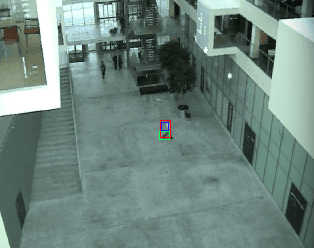
\includegraphics[width=0.8\linewidth]{groundfloorboxes}
  \caption{}
  \label{fig:persontracking1}
\end{subfigure}
\begin{subfigure}{1\textwidth}
  \centering
  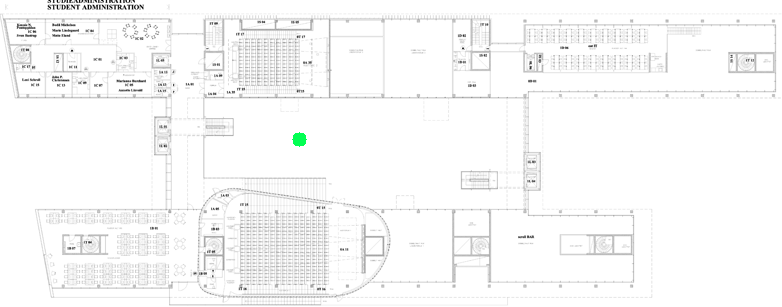
\includegraphics[width=0.8\linewidth]{maplocation}
  \caption{}
  \label{fig:persontracking2}
\end{subfigure}
\caption{The green dot on the map, corresponds to the position of the green box in the video frame.}
\label{fig:persontracking}
\end{figure}


It is important to note, that this approach only holds for movement within a plane, so when the subject in the video starts moving up the stairs, he leaves the plane that is the floor of the atrium, and the overview map coordinates stops being accurate. In the actual sequence, this is hard to detect, because the stairs have a very small slope.

A video of the views in Figure \ref{fig:persontracking} (a) and (b) called \texttt{displaytrace.mp4} can be found on the enclosed DVD

\section{Linear texture mapping}
\label{sec:linear}
\subsection*{Texture mapping on static object}
The function \texttt{textmapGroundFloor} takes a texture an maps it to each frame of the sequence 'sunclipds.avi'. A homography is created using the four corners of the the texture, and four points in the sequence selected by clicking on the first frame. The result is a texture placed 'statically' in the sequence. Figure \ref{fig:floor} show two different frames from the sequence.

\begin{figure}[H]
\centering
\begin{subfigure}{.4\textwidth}
  \centering
  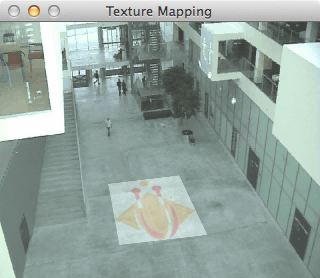
\includegraphics[width=0.8\linewidth]{groundfloor1}
  \label{fig:floor1}
\end{subfigure}
\begin{subfigure}{.4\textwidth}
  \centering
  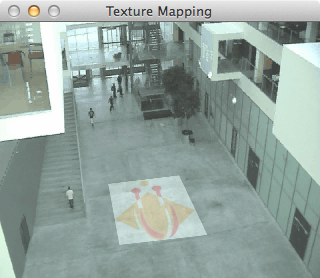
\includegraphics[width=0.8\linewidth]{groundfloor2}
  \label{fig:floor2}
\end{subfigure}
\caption{Linear texture mapping to sequence}
\label{fig:floor}
\end{figure}

\noindent
The function uses SIGBTools \texttt{getHomographyFromMousepoints} to create the homography, it should be noted that the order of the points are essential for the homography to work - the order of the four mouse clicks should be clockwise, the first point corresponds to the top left corner of the texture. Figure \ref{fig:floor_fail} illustrates the distortion as a result of click ordering.

\begin{figure}[H]
\centering
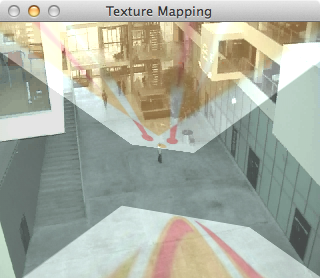
\includegraphics[width=0.32\linewidth]{floor_fail}
\caption{Distorted texture}
\label{fig:floor_fail}
\end{figure}




\section{Augmentation}
\label{sec:aug}
In the following, we will experiment with, and discuss, different techniques that can be used for augmenting images. (adding objects to an image that seems to behave as if real, with regards to perspective and position)
\subsection{Cameras and Calibration}
The camera matrix consists of two main parts, the intrinsic and the extrinsic parameters.

The extrinsic paramters describe the rotation and translation matrices needed to transform the objects in the world from world coordinates to the camera coordinates.

The intrinsic parameters describe the focal length, principal point, and format of the projection plane.

To find the calibration matrix, we capture a frame with a camera pointing at a chessboard figure, with a fixed square size of 2 centimeters.

The OpenCV function \texttt{calibrateCamera} can infer the focal length, the distortion coefficients, the translation and rotation matrix from the position of the chessboard squares.

\subsection{Camera Matrix via Homography}
%mw
After calibrating the camera, the following data is available. The camera matrix $K$, lists of rotation and translation vectors, one for each sample done in the calibration, the first frame of the samples and a set of points corresponding to the corners of the chess board in world coordinates.\\

The world coordinate system is defined according to the chessboard, meaning that the origin of the coordinate system is defined as the inner corner of one of the corner tiles of the chess board and that the chess board spans the $xy$-plane of the coordinate system. In other words all points that are on the same plane as the chess board in world coordinates are located in the $xy$-plane of the world coordinate system, meaning that for all of these points $z=0$.\\

Adding to this, that a frame in a video sequence is a 2D representation, meaning a plane, of the real world. This means that if we can find set corresponding points on the chess board and on the current frame, we can create a homography, which can be used to map any 2D structure on the the chess board to the current frame.\\

Because the transformation is from one plane to another the projection matrix $P_1$, from  the first sample in the calibration, which is known due to the calibration data, the two projection matrices can be related $P_2 = H P_1$ where $H = K[r_1,r_2,t]$, from this it is possible to calculate the third rotation vector $r_3 = r_1 \times r_2$ in the the rotation matrix $R$, meaning we can recalculate $P_2$, so that $z$ values in world coordinates can be mapped as well. By using $P_2$, which is calculated for each frame in a sequence, we can now map any point in world coordinates to that given frame. Figure \ref{fig:cube_from_homography} shows an image augmented with a cube in 3 dimensions, using this technique.\\


\begin{figure}[H]
\begin{centering}
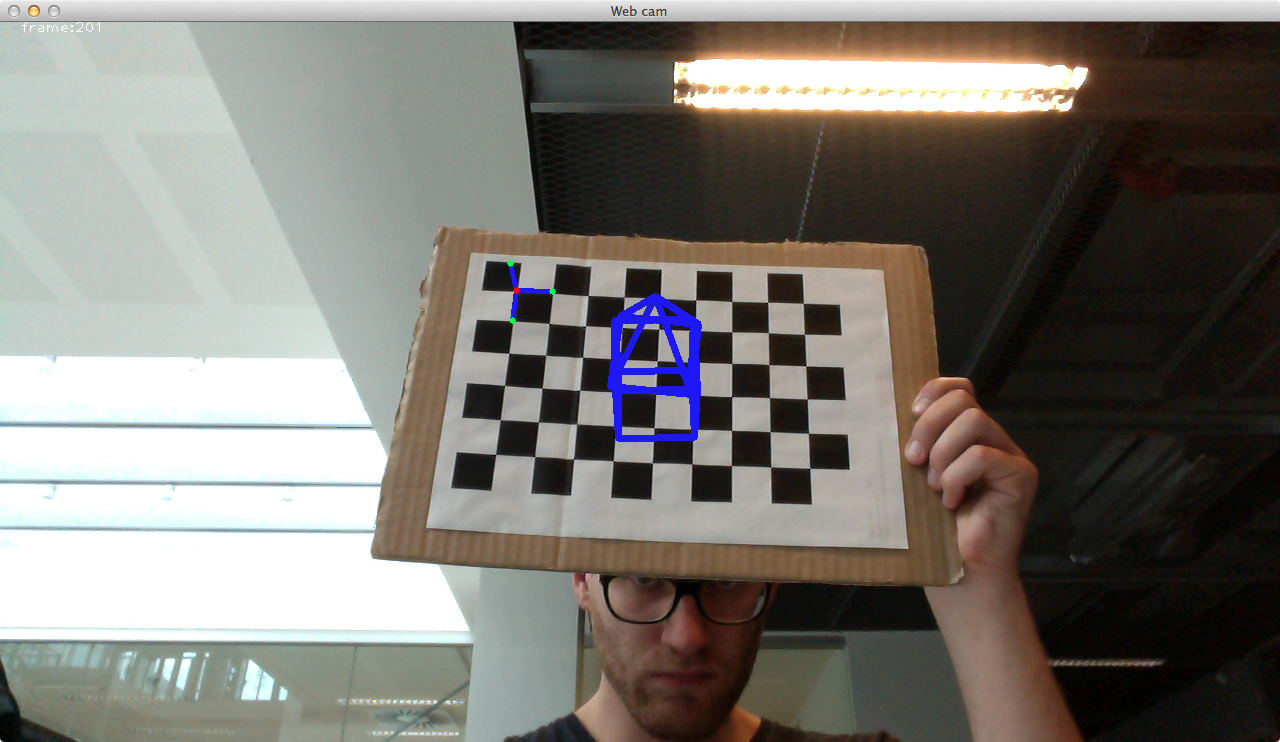
\includegraphics[width=0.8\linewidth]{cube_from_homography}
\caption{Augmented cube and pyramid using homography to find the current $P$}
\label{fig:cube_from_homography}
\end{centering}
\end{figure}

As figure \ref{fig:cube_from_homography} shows, the technique works, but at extreme angles the mapping of the $z$-coordinates fails, figure \ref{fig:cube_from_homography} shows this.\\


\begin{figure}[H]
\centering
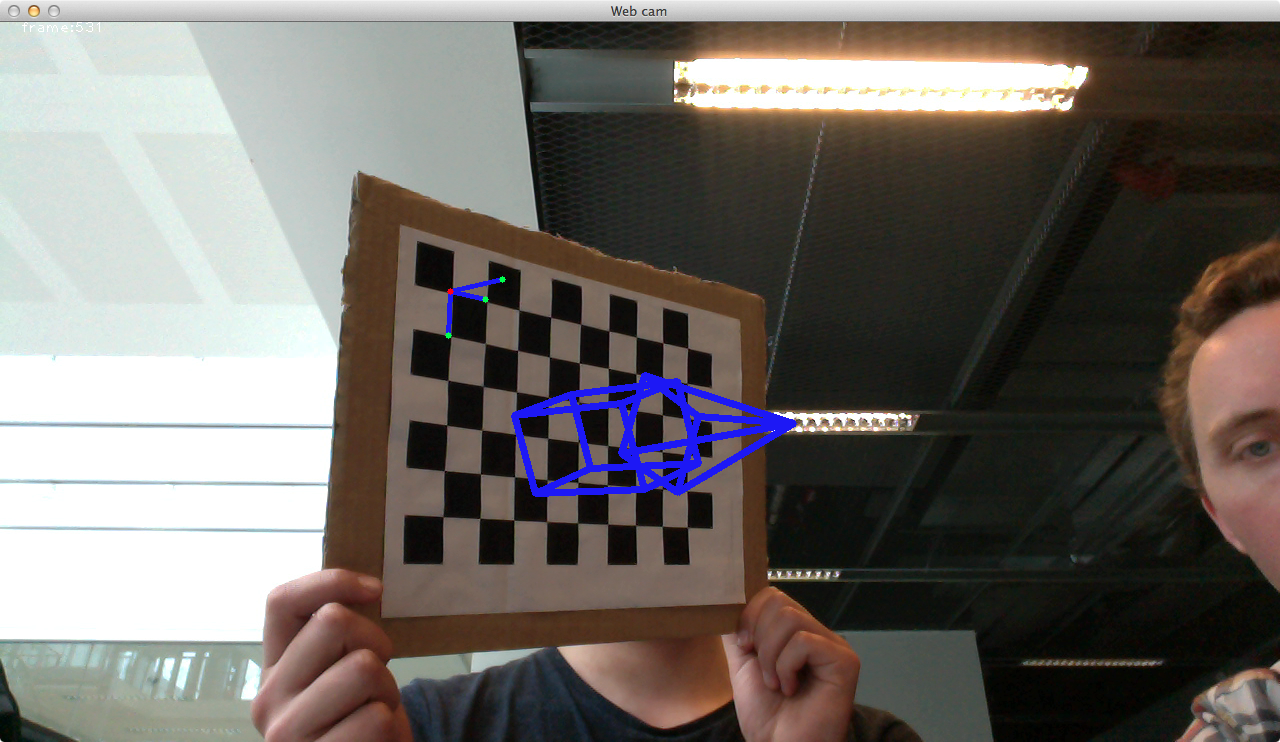
\includegraphics[width=0.8\linewidth]{cube_from_homography_fail}
\caption{Homography technique failing}
\label{fig:cube_from_homography_fail}
\end{figure}
\subsection{P from Object Pose}
%mf
The OpenCV function \texttt{solvePnP} can estimate the object "pose" (position and orientation in 3D space). To do this, it needs a set of points in the ChessBoard space $(x, y, z)$, the set of corresponding points in the image where we want to determine the pose $(x, y)$, and finally the camera matrix and distortion coefficients found via calibration. The result from \texttt{solvePnP}, is a rotation vector - $r_{vec}$, and a translation vector $t_{vec}$. The rotation vector can be converted to a rotation matrix, using the \texttt{Rodrigues} function.

Given the rotation matrix, $R$ the translation vector, $t$ and the camera matrix, $K$ we can determine P as: $P=K[R|t]$. This gives us a camera that allows us to project directly from the 3-dimensional ChessBoard space (not just plane), to any image where a chessboard pattern can be detected. Figure \ref{fig:cube_from_pose} shows an image augmented with a cube in 3 dimensions, using this technique.
\todo{indsæt figur}
The \texttt{solvePnP} technique appears to be extremely robust, and produces accurate results in all of our experiments.

\subsection{Comparison}
As mentioned in the previous sections, using homographies to calculate $P$, appear to be working in most cases, but at extreme angles the $z$-dimension if the object is distorted, whereas the object pose, appears robust in all our tests, the conclusion is therefore that the object pose technique is best.
%mw
%something about how homography vs object pose performs
%object pose appears to give more consistent results, also at extreme angles. blahhhhhhhh

\subsection{Alternative Objects}
%mw
The main challenge is calculating $P$ for the current frame, when this is achieved, it is possible to map any point in world coordinates to the current frame. We have implemented a function called \texttt{getPyramidPoints()}, which defines a pyramid, that can be drawn similarly to the cube. More generally, we have implemented \texttt{drawObjectScatter}, which takes a list of points in world coordinates.

Using this function we are able to draw a point cloud of the Utah teapot as shown in figure \ref{fig:teapot}
\begin{figure}[H]
\centering
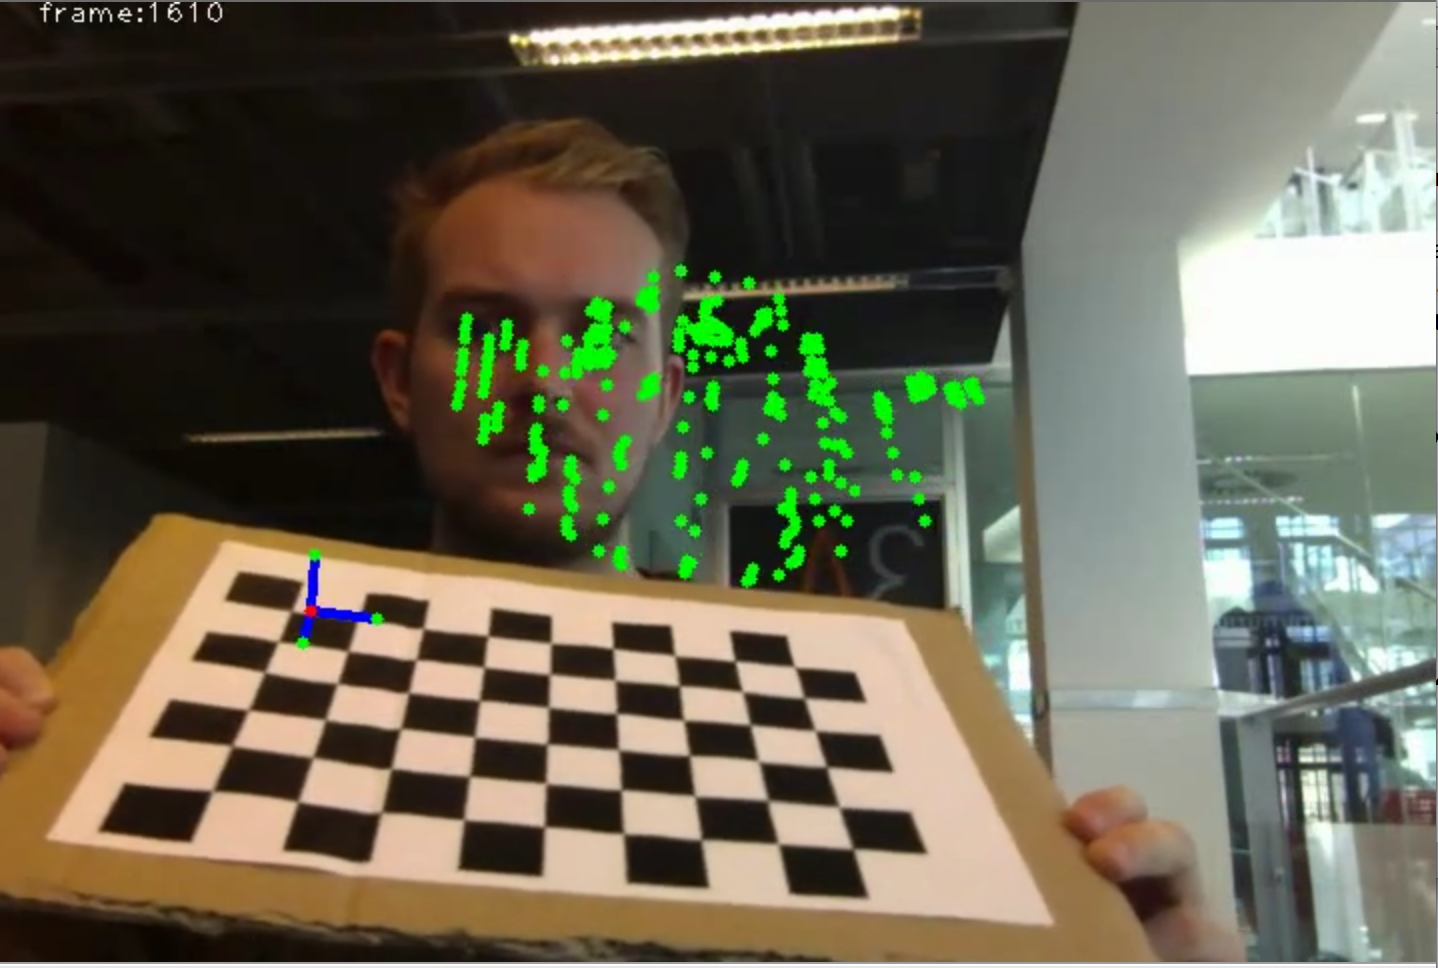
\includegraphics[width=0.6\linewidth]{teapot}
\caption{Augmenting the chessboard with the Utah teapot point cloud}
\label{fig:teapot}
\end{figure}

A point for further improvement, would be to add the possibility of drawing lines between corresponding points, thus being able to create a wireframe for any object.
\todo{toggle buttons?}
%pyramid, teapot, point-cloud rendering
%talk about wireframing
\subsection{Rotation, Scaling and Translation}
%mf
%potential todo: rewrite code so all 3 things happen in one matrix multiplication
Now that we can accurately project arbitrary points from the ChessBoard space onto any image where a chessboard can be found, we can easily transform the objects in ChessBoard coordinates, before projecting.

Our method \texttt{transformFigure} accepts as input: a set of points to be transformed, the amount to rotate around the 3 axes, the amount to scale each of the 3 axes by, and a translation vector, and gives as output the transformed points. (Rotation is achieved by using the 3-dimensional basic rotations, scaling by scalar multiplying and translation by addition).

To achieve animation, we can use the current framenumber as input to \texttt{transformFigure}, as follows.

\begin{lstlisting}
angle = frameNumber * (math.pi / 50.0)
scale = 2 + math.sin(angle)
\end{lstlisting}

The result of this, is that each frame will rotate the object by $\theta = \pi / 50$ radians, describing a full revolution every 100 frames. The scale of the object will vary smoothly between a factor 1 and a factor 3.

A recorded sequence, showcasing animations, transformations and alternative objects, can be found on the enclosed DVD in a file called 'animated\_alternative\_objects.mp4'

\section{Conclusion}
In this report we successfully found a homography from one plane to another, that allowed us to display tracking data from one plane, in the other.
\begin{itemize}
\item
We used the found homography to map textures onto planes in a realistic fashion, using transparency to heighten the illusion.
\item
We successfully calibrated a camera, and used this calibration (along with homographies or object poses) to perform real-time augmentation of a video-stream.
\item
We expanded the augmentation from a static image of a box, to include animations (rotation, scaling and translation) and multiple simultaneous, independent objects.
\item
We added a new object shape (a pyramid), and implemented point-cloud rendering - exemplified by a teapot.
\item
We compared two different methods for determining the projection matrix $P$, and found the one based on object pose to be superior in both precision and robustness.
\end{itemize}
We are especially proud of our work on animations, but would have liked to extend our point-cloud rendering to draw polygons, instead of just points.

\newpage
\section*{Appendix}
\subsection*{Assignment2.py}
\lstinputlisting[language=Python]{../ass2/Assignment2.py}
\subsection*{Assignment\_Cube.py}
\lstinputlisting[language=Python]{../ass2/Assignment_Cube.py}


\end{document}
